\newcommand{\Subject}{\textcolor{black}{Thesis Topics Defence}\\{---}\\\LARGE{Warped Hypertime,\\[0.2em] the Tool for Long-Term Autonomy}}
\newcommand{\Meeting}{MESAS 2018, Prague}
\newcommand{\Author}{Tom{\'a}{\v s} Vintr}
%\newcommand{\Authors}{Tom{\'a}{\v s} Vintr, Kerem Eyisoy, Vanda Vintrov{\'a}, Tom{\'a}{\v s} Krajn{\'i}k}
\newcommand{\Authors}{Tom{\'a}{\v s} Vintr}
\newcommand{\Date}{}
%\usetheme{warsaw}

\newcommand{\video}[2]{\href{run:#1}{\includegraphics[width=0.99\textwidth]{#2}}}
\newcommand{\link}[2]{\href{run:#1}{\includegraphics[width=0.99\textwidth]{#2}}}
\newcommand{\bib}[3]{\begin{thebibliography}{#1}\bibitem[#1]{#1}{#2}.\newblock{\em #3}\end{thebibliography}}

\newcommand{\Lincoln}{Artificial Intelligence Center\\Faculty of Electrical Engineering\\Czech Technical University}
\newcommand{\Institute}{\Lincoln\\}


\newcommand{\HeadLineLeft}{Tom{\'a}{\v s} Vintr}
\newcommand{\HeadLineCenter}{Thesis Topics Defence}
\newcommand{\HeadLineRight}{AIC@CTU}
\newcommand{\FootLineCenter}{Warped Hypertime, the Tool for Long-Term Autonomy}
\newcommand{\FootLineLeft}{\insertshortauthor}

\input{inc/head}

\title{{\bf \Subject}}
\usepackage{multirow}
\begin{document}
% - frame 1---------------------------------------------------------------------

\frame{\titlepage}

\begin{frame}
	\frametitle{SotA in Spatio-temporal Modelling}
    \vspace{3mm}
    \href{run:./video/MorseSpatioTemporalExploration.mp4}{\includegraphics[width=0.9\textwidth]{fig/The-robot-Linda-at-Open-space-office-and-Bob-at-office-corridor.png}}
\end{frame}


% - frame 2---------------------------------------------------------------------

\begin{frame}
	\frametitle{FreMEn in the Background}
    \vspace{3mm}
    \href{run:./video/pitch.mkv}{\includegraphics[width=0.9\textwidth]{fig/fremen_backgroung.jpeg}}
\end{frame}


% - frame 3---------------------------------------------------------------------

\begin{frame}
	\frametitle{Basic Assumtions for Model}
    \vspace{3mm}
    \begin{itemize}
        \item Human environment is stable in mid-term,
        \item changes are influenced mainly by human habits,
        \item behaviour before the midnight is identical to behaviour after the midnight,
        \item human is not a point mass.
    \end{itemize}
\end{frame}


% - frame 4---------------------------------------------------------------------

\begin{frame}
	\frametitle{WHyTe - Projection of Binary Variable}
    \vspace{3mm}
            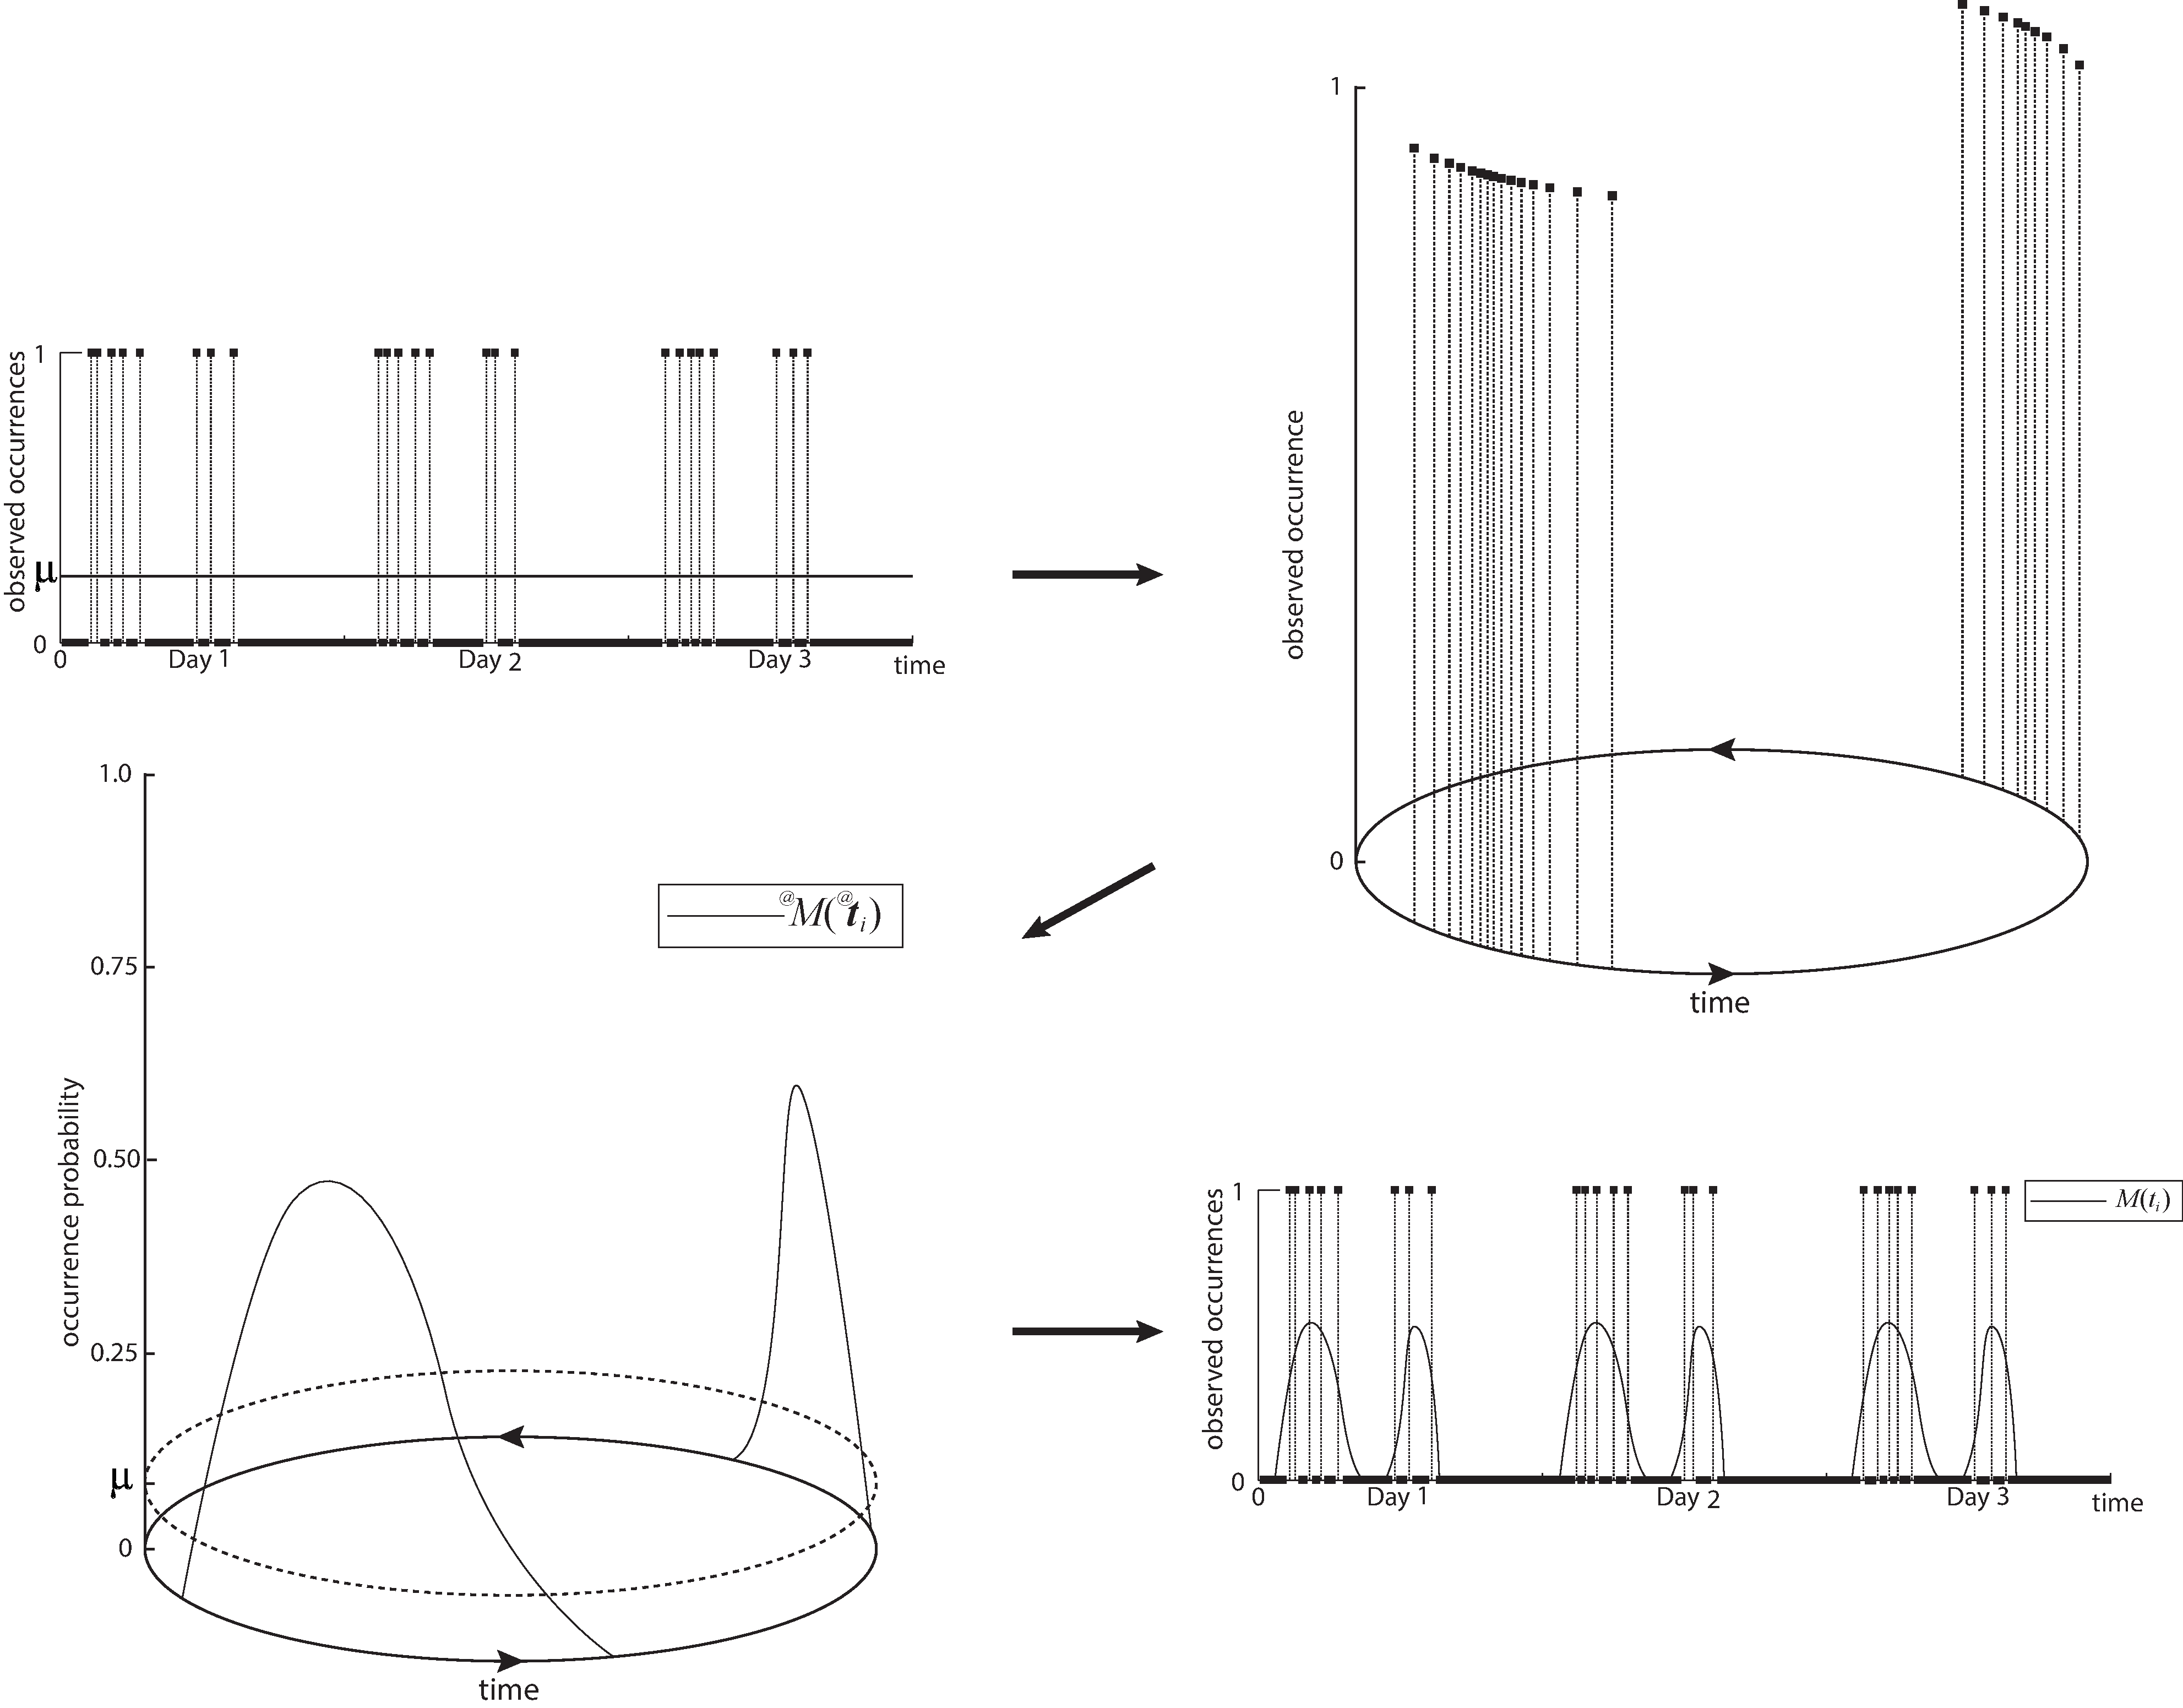
\includegraphics[width=0.9\textwidth]{fig/hypertime_graphs_a.pdf}
\end{frame}


% - frame 5---------------------------------------------------------------------

\begin{frame}
	\frametitle{WHyTeS - Projection of Vector Variable}
    \vspace{3mm}
            \includegraphics[width=0.8\textwidth]{fig/hypertime_space.pdf}
\end{frame}


% - frame 6---------------------------------------------------------------------

\begin{frame}
	\frametitle{FreMEn Model vs. WHyTe Model}
    \vspace{3mm}
            \includegraphics[width=0.8\textwidth]{fig/FreMEn_WHyTe.pdf}
\end{frame}



% - frame 7---------------------------------------------------------------------

\begin{frame}
	\frametitle{Prediction: WHyTe Power $\doteq$ FreMEn Power}
    \vspace{3mm}
\begin{figure}[!b]
   \begin{center}
      \includegraphics[width=0.45\columnwidth]{fig/door_graph}
    \hfill
      \includegraphics[width=0.45\columnwidth]{fig/localisation_graph}\\\vspace{5mm}
      \includegraphics[width=0.45\columnwidth]{fig/nav_graph}
    \hfill
      \includegraphics[width=0.45\columnwidth]{fig/ped_graph}
   \end{center}
\end{figure}
\end{frame}


% - frame 8---------------------------------------------------------------------

\begin{frame}
	\frametitle{Memory Efficiency of WHyTeS}
    \vspace{3mm}
\begin{table}[!b]
%\caption{Memory Efficiency of Compared Methods}
\label{tab:ram}
%\resizebox{1.0\textwidth}{!}{%
\centering{
\begin{tabular}{ccccc}
\hline
\begin{tabular}[c]{@{}c@{}}spatial\\cells\end{tabular} & \begin{tabular}[c]{@{}c@{}}WHyTeS\\ c = 3, @ = 2\end{tabular} & \begin{tabular}[c]{@{}c@{}}FreMEn\\ f = 5\end{tabular} & \begin{tabular}[c]{@{}c@{}}Hist\\ h = 24\end{tabular} & Mean      \\ \hline
400                                                          & 1.7 KiB                                                                & 1.1 MiB                                                & 19.3 KiB                                              & 3.3 KiB   \\
1600                                                            & 1.7 KiB                                                                & 4.4 MiB                                                & 307.3 KiB                                             & 12.9 KiB  \\
10000                                                            & 1.7 KiB                                                                & 27.2 MiB                                               & 1.9 MiB                                               & 80.1 KiB  \\
40000                                                            & 1.7 KiB                                                                & 108.9 MiB                                              & 7.7 MiB                                               & 320.1 KiB \\ \hline
\end{tabular}%
}
\end{table}

\end{frame}



% - frame 9---------------------------------------------------------------------

\begin{frame}
	\frametitle{WHyTeS Model Visualisation}
    \vspace{3mm}
    \href{run:./video/WHyTeS_visualisation.mp4}{\includegraphics[width=0.7\textwidth]{fig/corridor_datasetb.png}}
\end{frame}

% - frame 10---------------------------------------------------------------------

\begin{frame}
    \frametitle{Objectives}
    \vspace{3mm}
This research aims to create a universal tool based on the warped hypertime projection for the complex control of the autonomous robot in dynamic, human-populated environments and to deploy warped hypertime based methods on a real robot.
\end{frame}


% - frame 11---------------------------------------------------------------------

\begin{frame}
	\frametitle{Is It Even Possible?}
    \vspace{3mm}
\begin{figure}[!b]
   %\begin{center}
      \includegraphics[width=0.6\columnwidth]{fig/wars.jpg}
   %\end{center}
\end{figure}
\begin{figure}[!b]
   %\begin{center}
    \hspace{5mm}
      \includegraphics[width=0.6\columnwidth]{fig/Sunspot_Numbers.png}
   %\end{center}
\end{figure}
\end{frame}


% - frame ---------------------------------------------------------------------
\begin{frame}
	\frametitle{Questions}
	\begin{center}
		%\vfill
		%Code, paper and data available: \textbf{bearnav.eu}
		\vfill
		Thank you for your attention.\\
		\vfill
		Questions?
		\vfill
		\vfill
		\vfill
Many thanks go to my friends who participate on this work: Tomas Krajnik, Kerem Eysoi, Jiri Ulrich, Vanda Vintrova, Filip Mayer, Tomas Roucek, Lucie Halodova, George Broughton and Jan Faigl.
	\end{center}
\end{frame}


\end{document}
